\subsection{Fin de vía y transiciones}
    \label{sec:bufferstop}

    El tendido ferroviario no puede continuar de forma indefinida, ni tampoco interrumpirse de forma abrupta. Como se puede visualizar en la Figura \ref{fig:frontera_1}, existen dos formas de definir el fin de vía: de forma relativa y de forma absoluta.

    \begin{figure}[!h]
        \centering
        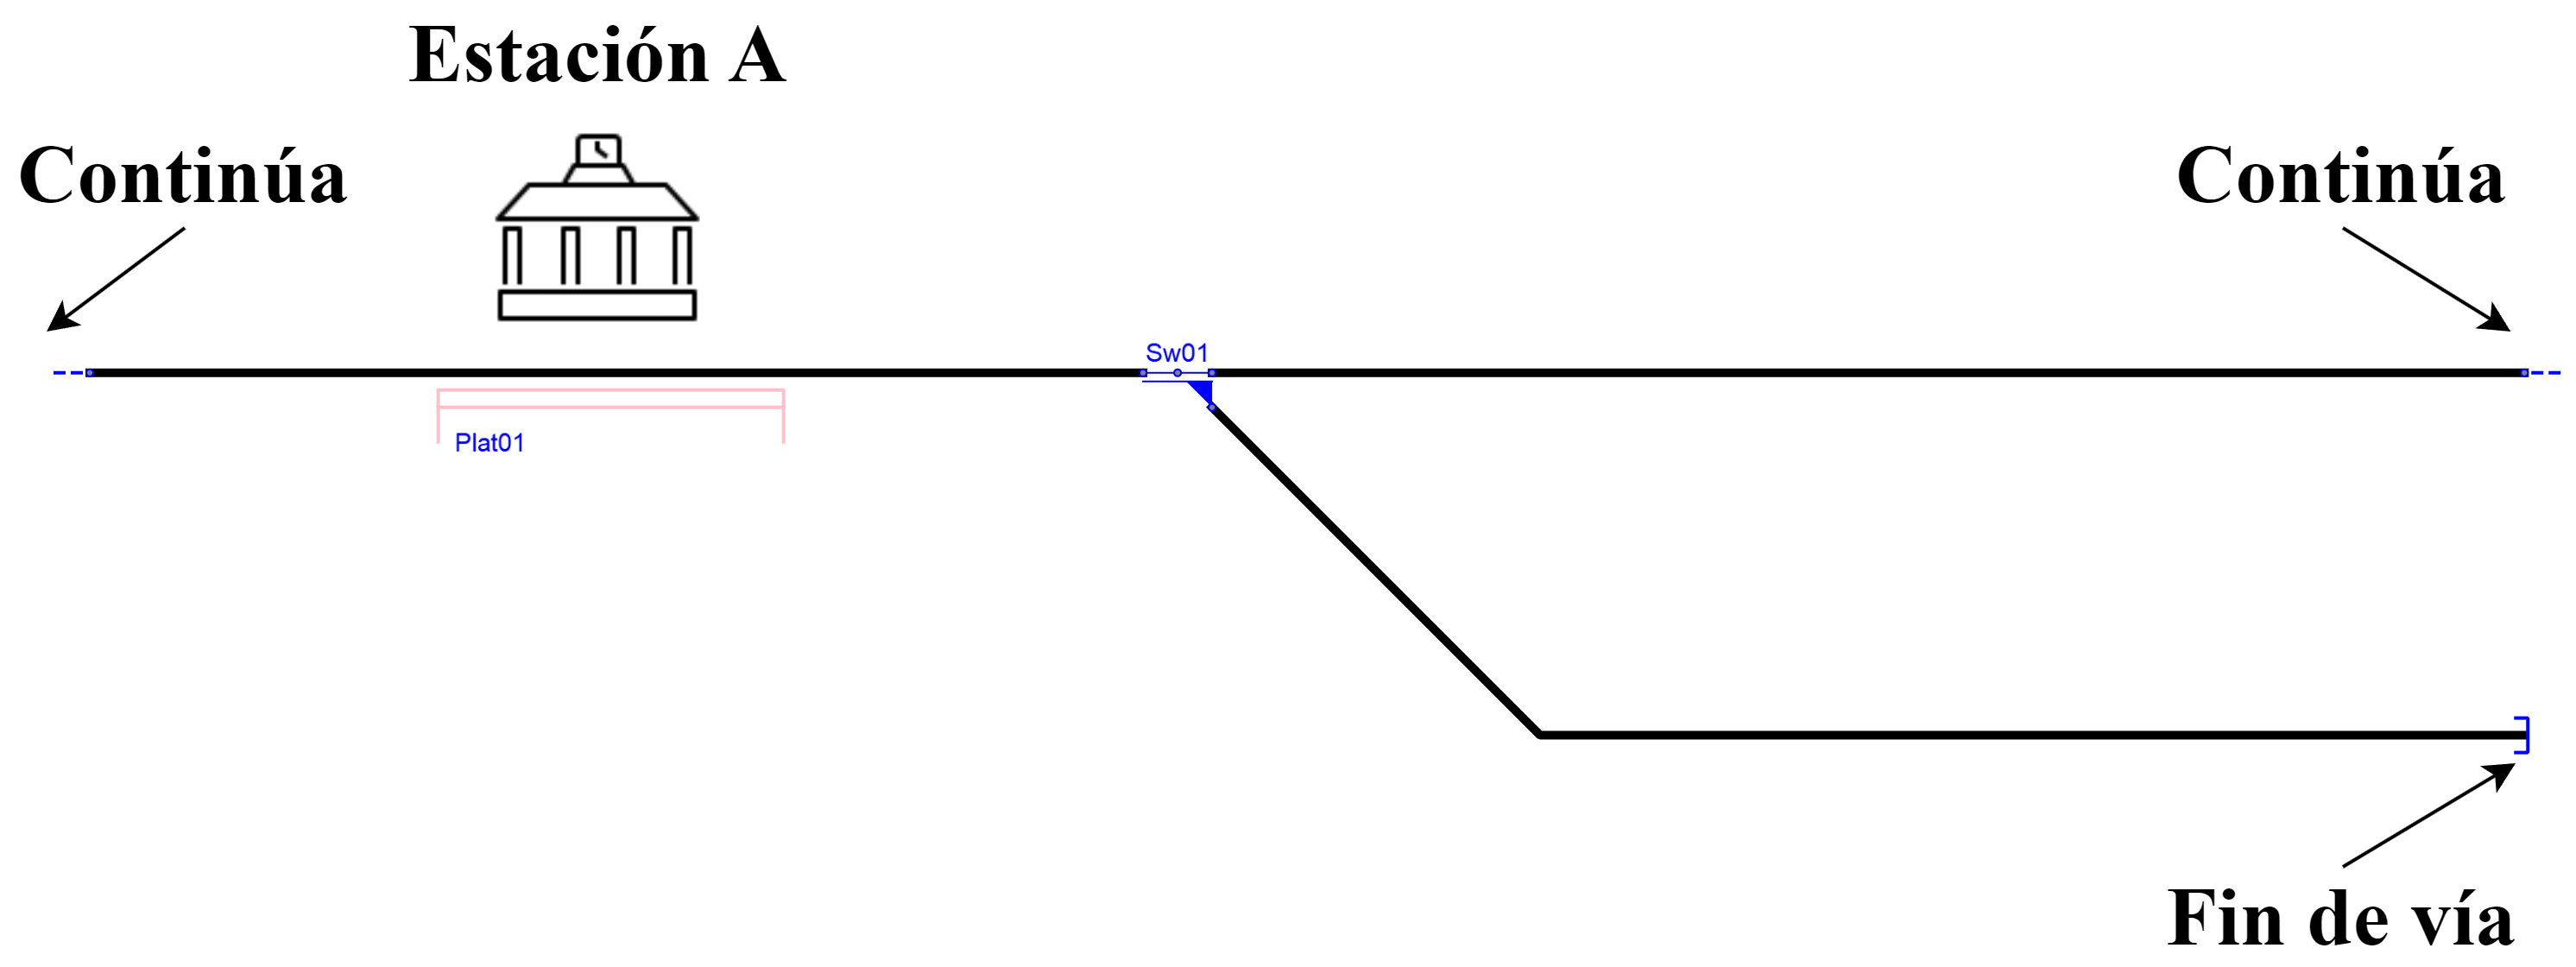
\includegraphics[width=0.9\textwidth]{Figuras/Border.png}
        \centering\caption{Topología de ejemplo con finales de vía relativos y absolutos.}
        \label{fig:frontera_1}
    \end{figure}

    Un ejemplo de fin de vía relativo sería la frontera entre las estaciones A y B. Las vías continúan a la derecha de A, pero no son parte del alcance del sistema que controla los elementos ferroviarios en las inmediaciones de A. En tanto que un fin de vía absoluto sería todo final literal de la red ferroviaria, tales como terminales, talleres y vías secundarias sin retorno, como la ramificación saliente de la vía principal.
    
    Un fin de vía relativo es todo aquel límite que define el alcance del sistema de señalamiento, pero no necesariamente es el final de la red. Es decir, el sistema podrá recibir información de cualquier sensor dentro de estos límites, o incluso de algunos sensores en la frontera exterior, pero solo podrá comandar los actuadores dentro de la zona. Esto es de vital importancia a la hora de reducir la complejidad de la red, al realizar el procesamiento de forma distribuida, sin depender de un decisión centralizada.

    Este elemento ferroviario es modelo por la clase border, cuyo ejemplo se visualiza en el Código \ref{lst:lineBorder}. Siempre se definen referido a un único netElement, en este caso el netElement ne114 y a una coordenada intrínseca que puede ser 0 si se encuentra al principio del netElement, o de 1 si se encuentra al final.

    \begin{lstlisting}[language = XML, caption = Clase border , label = {lst:lineBorder}]
    <border isOpenEnd="false" externalRef="" type="station" id="sb540">
        <designator register="_Example" entry="BORDER SB05"/>
        <spotLocation netElementRef="ne114" intrinsicCoord="0.0000" applicationDirection="reverse" id="sb540_sloc01"/>
        <name name="SB05" language="en"/>
    </border>
    \end{lstlisting}

    Un fin de vía absoluto es todo aquel límite que define el final físico del tendido ferroviario, luego del cual ya no se tiene infraestructura. Podemos encontrar estos límites en los talleres ferroviarios, en las terminales principales de cada red o en vías utilizadas para estacionar los trenes por fuera de la rama principal en uso. Estos límites deben estar adecuadamente protegidos y señalizados.

    Este elemento ferroviario es modelo por la clase bufferStop, cuyo ejemplo se visualiza en el Código \ref{lst:bufferStop}. Al igual que la clase border, se definen referido a un único netElement, en este caso el netElement ne3 y a una coordenada intrínseca que puede ser 0 si se encuentra al principio del netElement, o de 1 si se encuentra al final.
    
    \begin{lstlisting}[language = XML, caption = Clase bufferStop , label = {lst:bufferStop}]
    <bufferStop type="fixedBufferStop" id="bus5">
        <designator register="_Example" entry="BUFFERSTOP Buf05"/>
        <spotLocation netElementRef="ne3" intrinsicCoord="0.0000" applicationDirection="reverse" id="bus5_sloc01"/>
        <name name="Buf05" language="en"/>
    </bufferStop>
    \end{lstlisting}